\documentclass[../main.tex]{subfiles}
\begin{document}

In Abbildung \ref{fig:Kastengrafik} ist eine Kastengrafik zu sehen, die im folgenden zur Analyse der Umfrageergebnisse genutzt wird.
Die Grafik ist nach Kastengrafik-Konvention aufgebaut und ermöglicht einen Einblick in die Verteilung der Bewertungsergebnisse \autocite{williamson1989box} berechnet durch pgfplots \autocite{feuer2015manal}.
Der Bewertungsdurchschnitt wird zusätzlich in rot gezeichnet angezeigt.
\begin{figure}[h!]
\centering
\label{fig:Kastengrafik}
\begin{tikzpicture}
    \begin{axis}[
        boxplot/draw direction=y,
        x=0.82cm,
        ytick={1,...,5},
        xtick={1,...,15},
        xticklabel=\pgfmathprintnumber{\tick},
        axis x line*=bottom,
        axis y line*=left,
        xlabel={Fragen},
        ylabel={Bewertung},
        enlarge x limits,
        boxplot/average={auto},
        boxplot/every average/.style={mark=diamond*},
        /pgfplots/boxplot/hide outliers,
        fill=red
        ]
        \addplot [boxplot] table[y index=0] {data.dat};
        \addplot [boxplot] table[y index=1] {data.dat};
        \addplot [boxplot] table[y index=2] {data.dat};
        \addplot [boxplot] table[y index=3] {data.dat};
        \addplot [boxplot] table[y index=4] {data.dat};
        \addplot [boxplot] table[y index=5] {data.dat};
        \addplot [boxplot] table[y index=6] {data.dat};
        \addplot [boxplot] table[y index=7] {data.dat};
        \addplot [boxplot] table[y index=8] {data.dat};
        \addplot [boxplot] table[y index=9] {data.dat};
        \addplot [boxplot] table[y index=10] {data.dat};
        \addplot [boxplot] table[y index=11] {data.dat};
        \addplot [boxplot] table[y index=12] {data.dat};
        \addplot [boxplot] table[y index=13] {data.dat};
        \addplot [boxplot] table[y index=14] {data.dat};
    \end{axis}
\end{tikzpicture}
\caption{Kastengrafik zur Antwortverteilung}
\end{figure}
\begin{center}
    \begin{tikzpicture}
        \begin{axis}[
            width=10cm,
            view={60}{45},
            zmin=-0.001,
            area plot/.style={
                fill opacity=0.6,
                draw=cyan!80!black,
                fill=cyan,
                mark=none,
            },
            ytick={1,...,15},
            yticklabel=Q\pgfmathprintnumber{\tick},
        ]
        \pgfplotsinvokeforeach{8,7,...,1}{
            \addplot3 [area plot] table [
                x expr=\coordindex, y expr=#1, z=Q#1,
            ] {data3d.dat} \closedcycle;
        }
        \end{axis}
    \end{tikzpicture}
\end{center}
\begin{figure}[h!]
\centering
\label{fig:bereichdurchschnitt}
    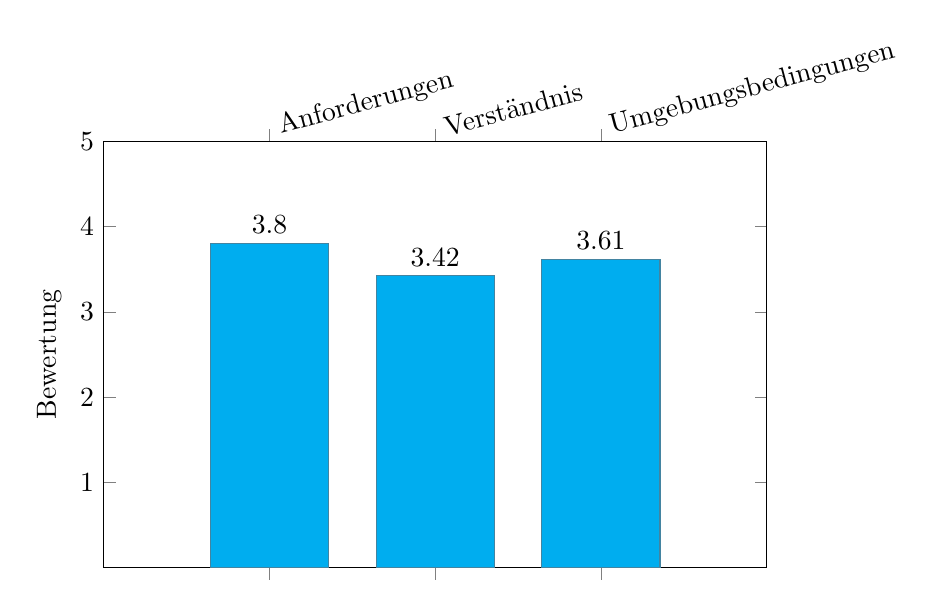
\begin{tikzpicture}
        \begin{axis}[
           ybar,
           symbolic x coords={a,Anforderungen, Verständnis, Umgebungsbedingungen,z},
           bar width={1.5cm},
           width={10cm},
           height={7cm},
           ylabel={Bewertung},
           x tick label style={anchor={west},rotate=15},
           xticklabel pos=upper,
           xtick=data,
           ytick={1,...,5},
           ymax=5,
           ymin=0,
           xmin={a},
           xmax={z},
           nodes near coords,
        ]
       \addplot[fill=cyan, draw=cyan!60!black] coordinates {
        (Anforderungen,3.8) (Verständnis,3.422222222) (Umgebungsbedingungen,3.613445378)
        };
        \end{axis}
    \end{tikzpicture}
\caption{durchschnittliche Bewertung nach vorgestellten Bereichen}
\end{figure}


\end{document}


